\section{Op Amp 741}
\begin{frame}{Op Amp 741}
	\begin{itemize}
		\item Monolitic amp $ \mu\text{A709} $ tahun 1965 oleh Fairchild Semiconductor
		\item $ \mu\text{A709} $ memiliki kekurangan $ \rightarrow $ dibuatlah $ \mu\text{A741} $
		\item Banyak manufaktur yang membuat $ \mu\text{A741} $:
		\begin{itemize}
			\item ON Semiconductor: MC1741
			\item Texas Instruments: LM741
			\item Analog Devices: AD741.
		\end{itemize}
		\item Istilah umumnya op amp 741
	\end{itemize}
\end{frame}

\subsection{Standar Industri}
\begin{frame}{Standar Industri}
	\begin{itemize}
		\item Beberapa versi: 741, 741A, 741C, 741E, dan 741N
		\item Bergantung pada karakteristiknya (voltage gain, temp. range, noise level, dll)
		\item 741C (C = \textit{Commercial grade}) $ \rightarrow $ sedikit lebih murah dan paling banyak digunakan
		\item $ A_{VOL} = 100000 $, $ z_{in} = 2 \text{ M}\Omega $, $ z_out = 75~\Omega $
	\end{itemize}
\end{frame}

\begin{frame}{Standar Industri}
	\begin{figure}
		\centering
		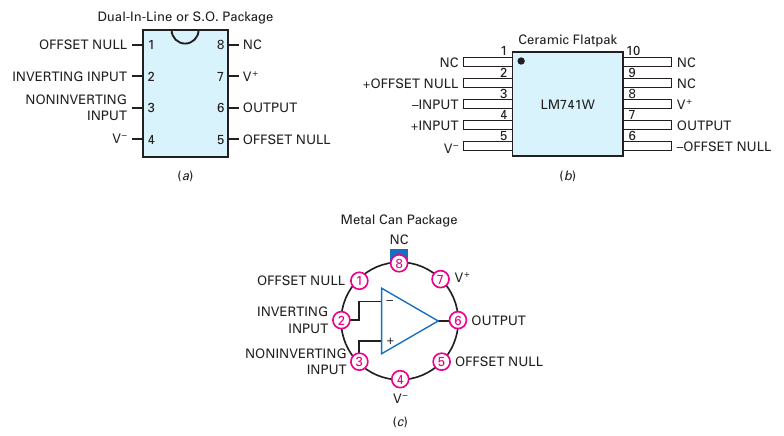
\includegraphics[width=0.7\linewidth]{gambar/fig-16.03}
		\caption{Op amp 741 pinouts (a) dual-in-line, (b) ceramic flatpak, (c) metal can}
		\label{fig-16.03}
	\end{figure}
\end{frame}

\subsection{Rangkaian Ekivalen dari Op Amp 741}
\begin{frame}{Rangkaian Ekivalen dari Op Amp 741}
	\begin{multicols}{2}
		\begin{figure}
			\centering
			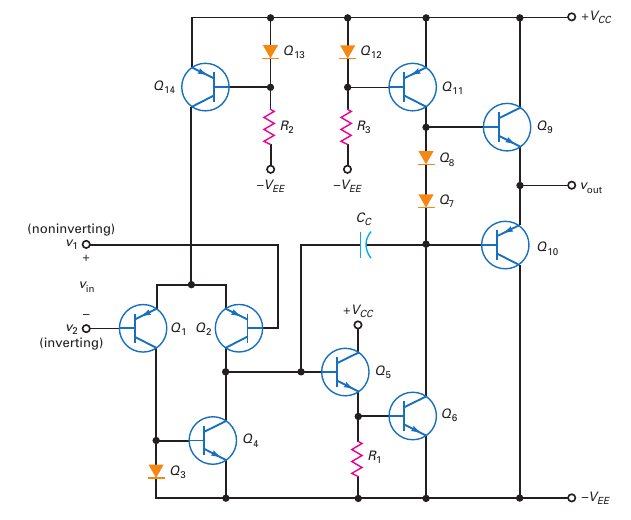
\includegraphics[width=0.9\linewidth]{gambar/fig-16.04}
			\caption{Rangkaian ekivalen dari op amp 741}
			\label{fig-16.04}
		\end{figure}
		\columnbreak
		\begin{itemize}
			\item Input diff amp
			\item Final Stage
			\item Active Loading
			\item Frequency Compensation $ C_{in(M)} = (A_v + 1) C_c $
		\end{itemize}
		\begin{figure}
			\centering
			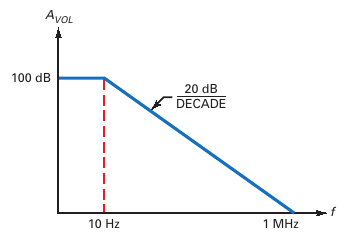
\includegraphics[width=0.5\linewidth]{gambar/fig-16.05}
			\caption{Bode plot $ A_{VOL} $ 741C ideal}
			\label{fig-16.05}
		\end{figure}
	\vfill\null
	\end{multicols}
\end{frame}

\subsection{Bias \& Offset}
\begin{frame}{Bias \& Offset}
	\begin{multicols}{2}
		\begin{figure}
			\centering
			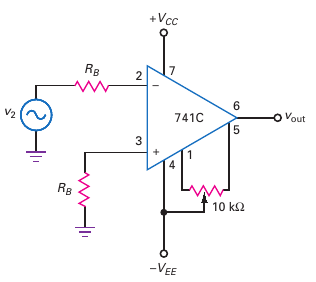
\includegraphics[width=0.8\linewidth]{gambar/fig-16.06}
			\caption{Penggunaan compensation dan nulling 741C}
			\label{fig-16.06}
		\end{figure}
		\columnbreak
		\begin{itemize}
			\item Tidak ada input signal $ \rightarrow $ input bias dan offset $ \rightarrow $ error output
			\item Error output berkurang $ \leftarrow $ base resistor yang sama $ \rightarrow $ hanya menghilangkan arus bias tapi tidak arus offset dan tegangan offset
			\item Solusi: menggunakan rangkaian nulling di datasheet
		\end{itemize}
		\vfill\null
	\end{multicols}
\end{frame}

\subsection{CMRR, MPP, dan $A_{VOL}$}
\begin{frame}{CMRR, MPP, dan $A_{VOL}$}
	\begin{figure}
		\centering
		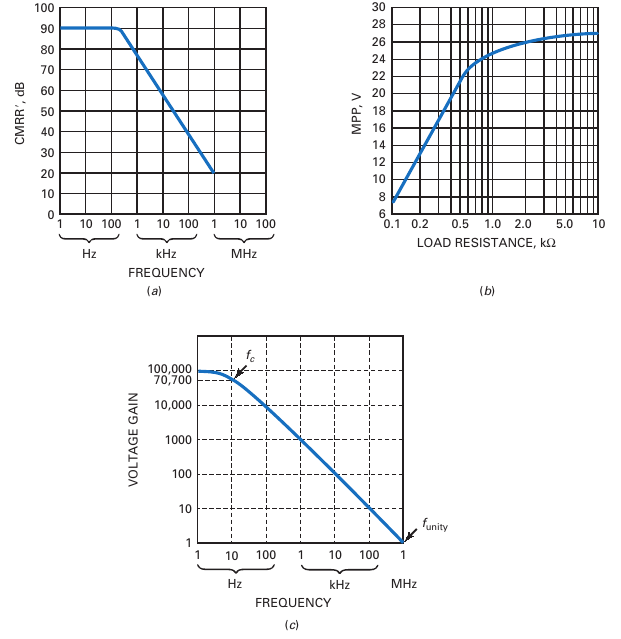
\includegraphics[width=\linewidth]{gambar/fig-16.07}
		\caption{Grafik (a) Common-Mode Rejection Ratio (CMRR), (b) Maximum Peak-to-Peak Output (MPP), dan (c) Open-Loop Voltage Gain $A_{VOL}$ dari 741C}
		\label{fig:fig-07}
	\end{figure}
	\vfill\null
\end{frame}

\subsection{Slew Rate}
\begin{frame}{Slew Rate}
	\begin{multicols}{2}
		\begin{figure}
			\centering
			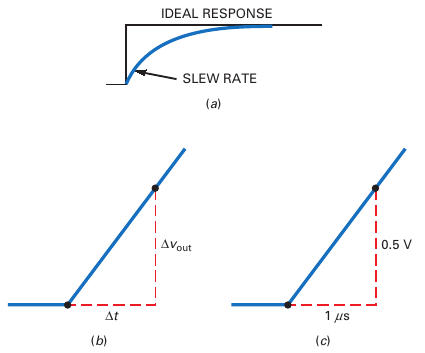
\includegraphics[width=0.8\linewidth]{gambar/fig-16.08}
			\caption{(a) Respon ideal dan aktual terhadap tegangan step input, (b) ilustrasi definisi slew rate, (c) $ S_R = 0.5 \text{ V/}\mu\text{s} $}
			\label{fig:fig-08a}
		\end{figure}
		\columnbreak
		\begin{itemize}
			\item Persamaan slew rate, $ S_R $
			\begin{equation}\label{pers.1}
				S_R = \frac{\Delta v_{out}}{\Delta t}
			\end{equation}
			\item Exponential wave meningkat 0.5 V selama 1 mikrodetik pertama:
			\begin{align*}
				S_R &= \frac{\Delta v_{out}}{\Delta t} \\
				&= \frac{0.5 \text{ V}}{1~\mu\text{s}} \\
				&= 0.5 \text{ V/}\mu\text{s}
			\end{align*}
		\end{itemize}
	\end{multicols}
\end{frame}

\begin{frame}{Slew Rate}
	\begin{figure}
		\centering
		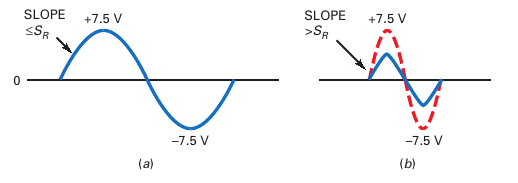
\includegraphics[width=\linewidth]{gambar/fig-16.09}
		\caption{(a) Initial slope dari gelombang sinus, (b) distorsi terjadi jika initial slope melebihi slew rate}
		\label{fig-16.09}
	\end{figure}
\end{frame}

\begin{frame}{Slew Rate}
	\begin{itemize}
		\item Sinyal dan frekuensinya sangat kecil $ \rightarrow $ slew rate bukan masalah
		\item Sinyal dan frekuensinya sangat besar $ \rightarrow $ slew rate akan mendistorsi sinyal ouput
		\[ S_S = 2 \pi f V_p \]
		\item $ S_s $: initial slope dari gelombang sinus, $ f $: frekuensi, $ V_p $: nilai peak
		\begin{align*}
			S_S &\leq S_R \\
			2 \pi f V_p &\leq S_R \\
			f &\leq \frac{S_R}{2 \pi V_p} \\
		\end{align*}
		\begin{equation} \label{pers.16.2}
			f_{max} = \frac{S_R}{2 \pi V_p}
		\end{equation}
	\end{itemize}
\end{frame}

\begin{frame}{Slew Rate}
	\begin{multicols}{2}
		\begin{figure}
			\centering
			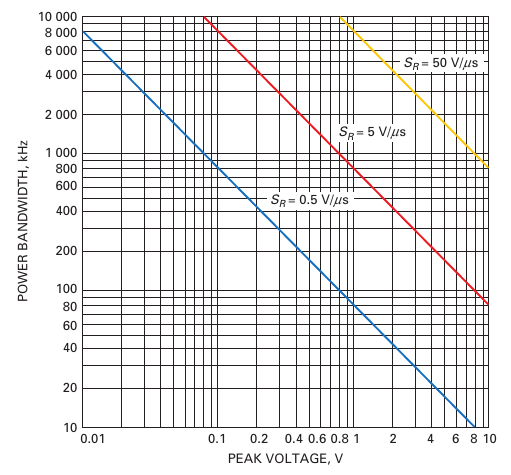
\includegraphics[width=0.8\linewidth]{gambar/fig-16.10}
			\caption{Grafik power bandwidth vs. peak voltage}
			\label{fig-16.10}
		\end{figure}
		\columnbreak
		\begin{itemize}
			\item  $ f_{max} $: power bandwidth atau large-signal bandwidth
			\item $ S_R = 0.5 \text{ V/}\mu\text{s} \rightarrow $ 741C
			\item $ S_R = 50 \text{ V/}\mu\text{s} \rightarrow $ LM318
		\end{itemize}
	\end{multicols}	
\end{frame}

\subsection{Contoh Soal 2.1}
\begin{frame}{Contoh Soal 2.1}
	\begin{multicols}{2}
		\begin{center}
			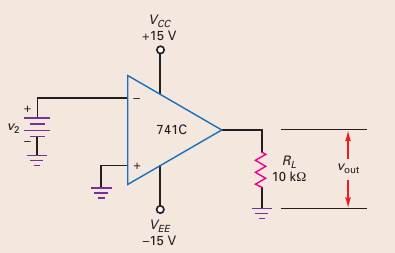
\includegraphics[width=\linewidth]{gambar/fig-16.11}
		\end{center}
		\columnbreak
		\begin{itemize}
			\item Pertanyaan:
			\begin{itemize}
				\item Berapa tegangan inverting input yang dibutuhkan untuk men-drive op amp 741C hingga saturasi negatif?
			\end{itemize}
		\end{itemize}
	\end{multicols}
\end{frame}